\documentclass[bachelor, och, labwork]{shiza}
% параметр - тип обучения - одно из значений:
%    spec     - специальность
%    bachelor - бакалавриат (по умолчанию)
%    master   - магистратура
% параметр - форма обучения - одно из значений:
%    och   - очное (по умолчанию)
%    zaoch - заочное
% параметр - тип работы - одно из значений:
%    referat    - реферат
%    coursework - курсовая работа (по умолчанию)
%    diploma    - дипломная работа
%    pract      - отчет по практике
% параметр - включение шрифта
%    times    - включение шрифта Times New Roman (если установлен)
%               по умолчанию выключен
\usepackage{subfigure}
\usepackage{tikz,pgfplots}
\pgfplotsset{compat=1.5}
\usepackage{float}

%\usepackage{titlesec}
\setcounter{secnumdepth}{4}
%\titleformat{\paragraph}
%{\normalfont\normalsize}{\theparagraph}{1em}{}
%\titlespacing*{\paragraph}
%{35.5pt}{3.25ex plus 1ex minus .2ex}{1.5ex plus .2ex}

\titleformat{\paragraph}[block]
{\hspace{1.25cm}\normalfont}
{\theparagraph}{1ex}{}
\titlespacing{\paragraph}
{0cm}{2ex plus 1ex minus .2ex}{.4ex plus.2ex}

% --------------------------------------------------------------------------%


\usepackage[T2A]{fontenc}
\usepackage[utf8]{inputenc}
\usepackage{graphicx}
\graphicspath{ {./images/} }
\usepackage{tempora}

\usepackage[sort,compress]{cite}
\usepackage{amsmath}
\usepackage{amssymb}
\usepackage{amsthm}
\usepackage{fancyvrb}
\usepackage{listings}
\usepackage{listingsutf8}
\usepackage{longtable}
\usepackage{array}
\usepackage[english,russian]{babel}

% \usepackage[colorlinks=true]{hyperref}
\usepackage{url}

\usepackage{underscore}
\usepackage{setspace}
\usepackage{indentfirst} 
\usepackage{mathtools}
\usepackage{amsfonts}
\usepackage{enumitem}
\usepackage{tikz}

\newcommand{\eqdef}{\stackrel {\rm def}{=}}
\newcommand{\specialcell}[2][c]{%
\begin{tabular}[#1]{@{}c@{}}#2\end{tabular}}

\renewcommand\theFancyVerbLine{\small\arabic{FancyVerbLine}}

\newtheorem{lem}{Лемма}

\begin{document}

% Кафедра (в родительном падеже)
\chair{}

% Тема работы
\title{ЗНАКОМСТВО С ПРОГРАММОЙ-СИМУЛЯТОРОМ PACKET TRACER}

% Курс
\course{2}

% Группа
\group{231}

% Факультет (в родительном падеже) (по умолчанию "факультета КНиИТ")
\department{факультета КНиИТ}

% Специальность/направление код - наименование
%\napravlenie{09.03.04 "--- Программная инженерия}
%\napravlenie{010500 "--- Математическое обеспечение и администрирование информационных систем}
%\napravlenie{230100 "--- Информатика и вычислительная техника}
%\napravlenie{231000 "--- Программная инженерия}
\napravlenie{100501 "--- Компьютерная безопасность}

% Для студентки. Для работы студента следующая команда не нужна.
% \studenttitle{Студентки}

% Фамилия, имя, отчество в родительном падеже
\author{Окунькова Сергея Викторовича}

% Заведующий кафедрой
% \chtitle{} % степень, звание
% \chname{}

%Научный руководитель (для реферата преподаватель проверяющий работу)
\satitle{ассистент} %должность, степень, звание
\saname{А. А. Фомин}

% Руководитель практики от организации (только для практики,
% для остальных типов работ не используется)
% \patitle{к.ф.-м.н.}
% \paname{С.~В.~Миронов}

% Семестр (только для практики, для остальных
% типов работ не используется)
%\term{8}

% Наименование практики (только для практики, для остальных
% типов работ не используется)
%\practtype{преддипломная}

% Продолжительность практики (количество недель) (только для практики,
% для остальных типов работ не используется)
%\duration{4}

% Даты начала и окончания практики (только для практики, для остальных
% типов работ не используется)
%\practStart{30.04.2019}
%\practFinish{27.05.2019}

% Год выполнения отчета
\date{2021}

\maketitle

% Включение нумерации рисунков, формул и таблиц по разделам
% (по умолчанию - нумерация сквозная)
% (допускается оба вида нумерации)
% \secNumbering

%-------------------------------------------------------------------------------------------

\section{Задания}

\begin{enumerate}
    
    \item Запустите Packet Tracer и познакомьтесь с его интерфейсом.
    
    \begin{figure}[H]
        \centering      %размер рисунка       здесь находится название файла рисунка, без указания формата
        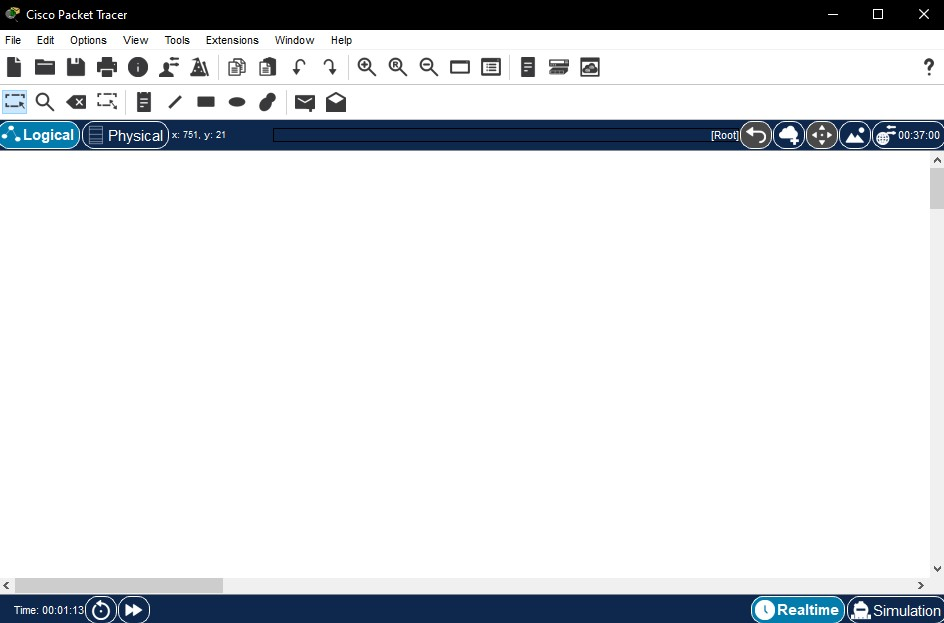
\includegraphics[width=1\textwidth]{1}
        \caption{Окно программы Packet Tracer}
        \label{fig:image1}
    \end{figure}

    \item Создайте конфигурацию, представленную на рисунке. Подключение компьютера к коммутатору выполните 
    консольным кабелем, используя порты RS-232 на компьютере и Console на коммутаторе:

    \begin{figure}[H]
        \centering      %размер рисунка       здесь находится название файла рисунка, без указания формата
        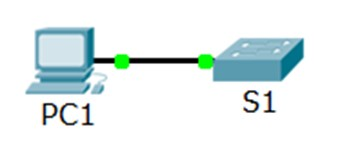
\includegraphics[width=0.5\textwidth]{2}
        \caption{Заданная конфигурация}
        \label{fig:image1}
    \end{figure}

    \begin{figure}[H]
        \centering      %размер рисунка       здесь находится название файла рисунка, без указания формата
        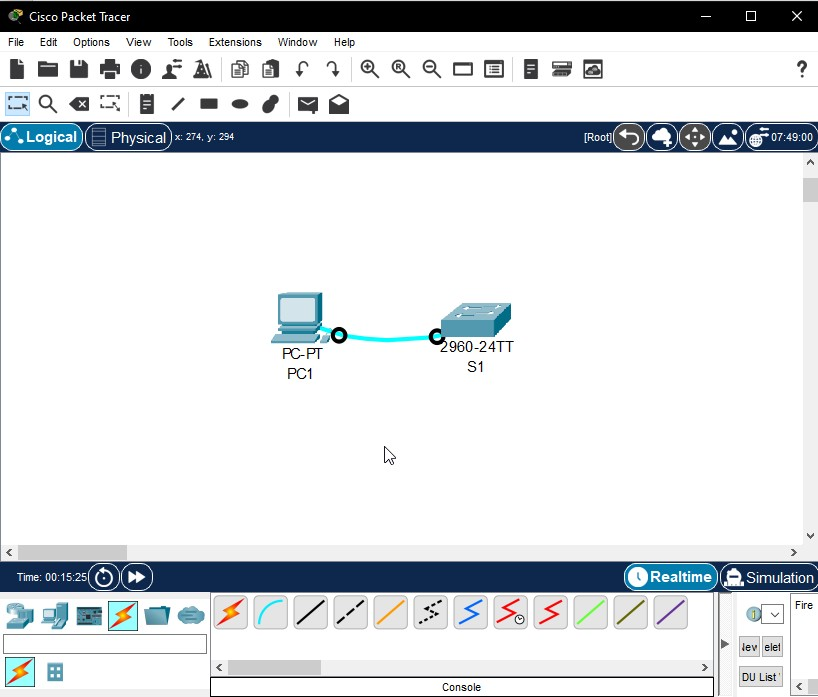
\includegraphics[width=1\textwidth]{3}
        \caption{Реализация заданной конфигурации в программе}
        \label{fig:image1}
    \end{figure}

    \item Воспользовавшись закладкой Desktop в окне настройки компьютера, запустите на нем терминальную программу.
    
    \begin{figure}[H]
        \centering      %размер рисунка       здесь находится название файла рисунка, без указания формата
        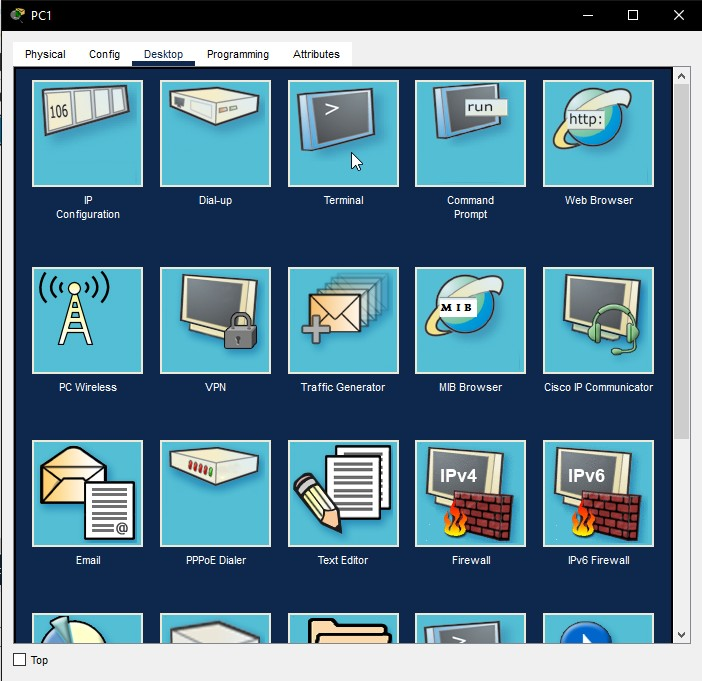
\includegraphics[width=0.75\textwidth]{4}
        \caption{Запуск терминальной программы}
        \label{fig:image1}
    \end{figure}

    \item Выполните подключение  с предложенными параметрами. Доступ к какому устройству вам предоставлен? Каков режим 
    доступа вы имеете, судя по виду приглашения командной строки? 

    Мы имеем глобальный режим доступа к коммутатору "Switch".

    \begin{figure}[H]
        \centering      %размер рисунка       здесь находится название файла рисунка, без указания формата
        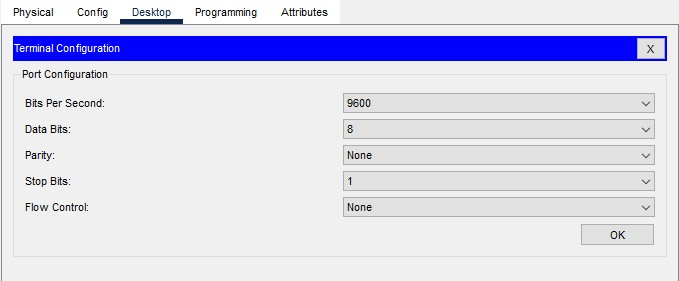
\includegraphics[width=0.75\textwidth]{5}
        \caption{Предложенные параметры терминальной программы}
        \label{fig:image1}
    \end{figure}

    \begin{figure}[H]
        \centering      %размер рисунка       здесь находится название файла рисунка, без указания формата
        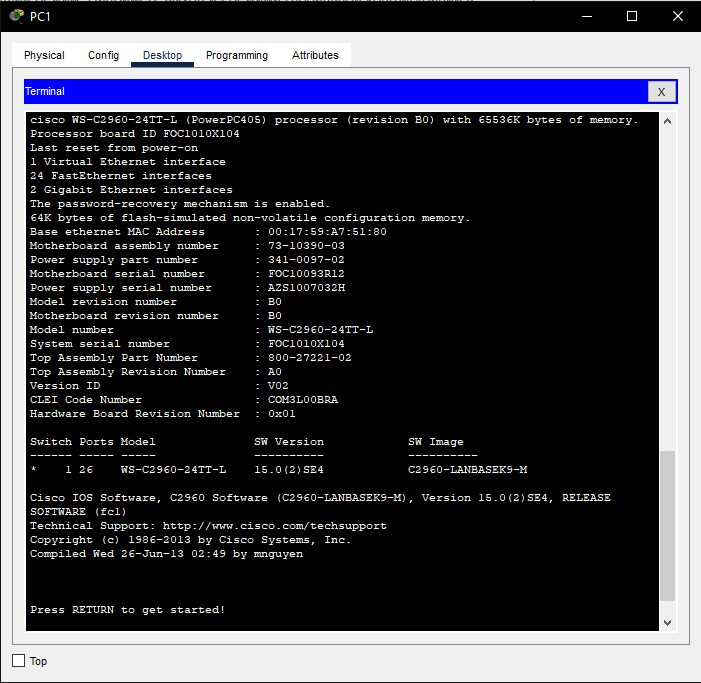
\includegraphics[width=0.75\textwidth]{6}
        \caption{Интерфейс терминала}
        \label{fig:image1}
    \end{figure}

    \item Введите команду S1>? Что является результатом её исполнения? Поочередно выполните команды S1>t? и S1>tel? Почему 
    результаты их исполнения различны?

    \begin{figure}[H]
        \centering      %размер рисунка       здесь находится название файла рисунка, без указания формата
        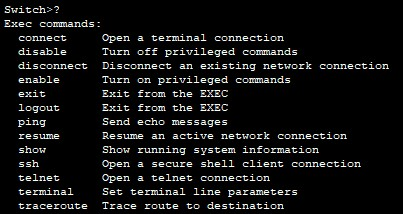
\includegraphics[width=1\textwidth]{7}
        \caption{Команда S1>?}
        \label{fig:image1}
    \end{figure}

    Результатом команды S1>? является список команд.

    \begin{figure}[H]
        \centering      %размер рисунка       здесь находится название файла рисунка, без указания формата
        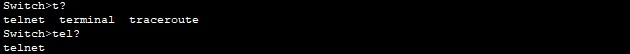
\includegraphics[width=1\textwidth]{8}
        \caption{Результаты команда S1>t? и S1>tel?}
        \label{fig:image1}
    \end{figure}

    У данных команд различный результат, потому что первая команда выдает список команд, начиняющихся с "t", а вторая
    - с "tel".

    \item Воспользовавшись командой S1>? выберите команду, позволяющую перейти в привилегированный пользовательский 
    режим. Введите  её первые два символа и нажмите клавишу "Tab", поясните результат.

    Команда, позволяющая перейти в привелигерованный пользовательский режим - "enable". При написание 2 символов и 
    нажатие на "tab", произойдет дополнение этих двух символов до самой команды.

    \item  Перейдите в привилегированный пользовательский режим. Что может свидетельствовать о том, что такой переход 
    выполнен успешно?

    Об успешном переходе в привелигерованный режим свидетельствует замена символа ">" на "\#" после S1.

    \item Что изменилось в выводе команды "?" ?
    
    \begin{figure}[H]
        \centering      %размер рисунка       здесь находится название файла рисунка, без указания формата
        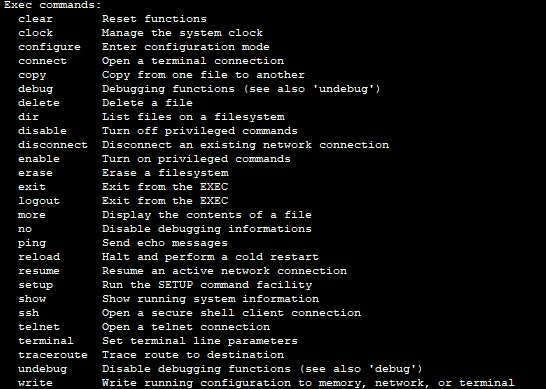
\includegraphics[width=1\textwidth]{9}
        \caption{Команда "?" в привелигерованном режиме}
        \label{fig:image1}
    \end{figure}

    Изменился список команд.

    \item Перейдите в глобальный конфигурационный режим. Поменяйте имя коммутатора с "S1" на "CSaIT311". 
    Вернитесь в привилегированный пользовательский режим. Что изменилось в приглашении командной строки?

    \begin{figure}[H]
        \centering      %размер рисунка       здесь находится название файла рисунка, без указания формата
        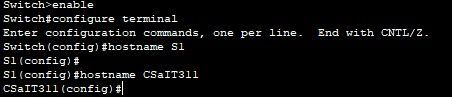
\includegraphics[width=1\textwidth]{10}
        \caption{Изменения, которые произошли из-за смены имени комутатора}
        \label{fig:image1}
    \end{figure}

    \item С помощью обращения к системе контекстной помощи через "?" определите текущее системное время. 
    Какое оно?

    \begin{figure}[H]
        \centering      %размер рисунка       здесь находится название файла рисунка, без указания формата
        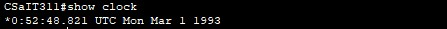
\includegraphics[width=1\textwidth]{11}
        \caption{Текущая дата и время}
        \label{fig:image1}
    \end{figure}

    \item Установите в системе правильное текущее время.
    
    \begin{figure}[H]
        \centering      %размер рисунка       здесь находится название файла рисунка, без указания формата
        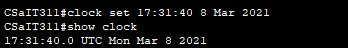
\includegraphics[width=1\textwidth]{12}
        \caption{Изменение даты и времени}
        \label{fig:image1}
    \end{figure}

    \item Определите тип коммутатора S1, количество портов и их тип.
    
    \begin{figure}[H]
        \centering      %размер рисунка       здесь находится название файла рисунка, без указания формата
        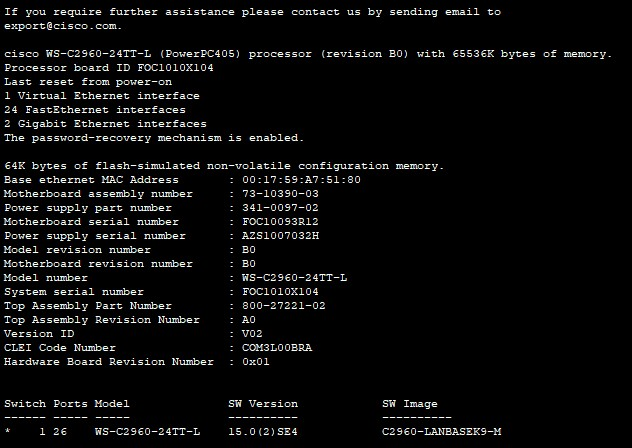
\includegraphics[width=1\textwidth]{13}
        \caption{Информация о коммутаторе S1}
        \label{fig:image1}
    \end{figure}

\end{enumerate}

\end{document}
